\documentclass[12pt]{article}
\usepackage[a4paper, total={5in, 9in}]{geometry}
\usepackage[utf8]{inputenc}
\usepackage{caption}
\usepackage{amsmath}
\usepackage{amssymb}
\usepackage{mathtools}
\usepackage{multicol}
\usepackage{graphicx}
\usepackage{wrapfig}
\usepackage{float}
\usepackage[makeroom]{cancel}
\usepackage{mhchem}

\graphicspath{ {../images/} }

\renewcommand{\baselinestretch}{1.5} % line spacing
\newcommand{\fline}{\par\noindent\rule{\textwidth}{0.1pt}} % horizontal line (wide)

\title{Dynamics Lab\\Acceleration with a Pulley}
\author{Peter Zhang}

\begin{document}

\maketitle
\pagebreak
\tableofcontents
\newpage

\section{What is Gibb's Free Energy}
It is the free energy in a system that can do useful work. The amount of \textbf{ENERGY in a system that is AVAILABLE to do USEFUL work}. Also known as standard free energy or free energy of a system!

\begin{itemize}
\item if we had a reaction that was happening and was exothermic (heat released), heat would be released out of the system.
\item if we trap all the heat (isolated system / calorimeter), the heat that is freed in the isolated system can be transferred back into the reaction
\item more energy is gone towards completion, more efficiency?
\item this can also have a `reverse effect` as the excess energy may reverse the reaction
	\begin{itemize}	
	\item reduces overall effect of the reaction
	\item `lower percent yield`
	\end{itemize}
\end{itemize}

\subsection{Isolated Systems}
Isolated systems are systems that essentially have no external factors that can affect the stuff inside.

\subsubsection{Pop Cans}
Take for example, pop cans. Carbonated drinks produce a lot of pressure and in pop cans, the gas flows in a circular cycle. The gas cycles out of the solution and back into the solution. This is what keeps the bubbling/carbonated pressure.


\section{Units of Gibbs Free Energy}

The units for Gibb's Free energy is 
$$\triangle{G} = kJ/mol$$

\section{Equation for Gibb's Free Energy}

\subsubsection{Given Enthalpy, Temperature, and Entropy}

$$\triangle{G} = \triangle{H}_{sys} - T\triangle{S}_{sys}$$

Usually when you calculate for $\triangle{G}$ you are also given the $\triangle{H}$, the $\triangle{S}$, and $T$ of a system. Plugging them into the formula above will give you the Gibb's Free Energy of a system at a certain temperature. Remember to convert the units for entropy!

\subsubsection{Given Data Booklet $\star$ \textbf{FOR REACTIONS}}

$$\triangle{G} = \sum{\triangle{G}_{products}} - \sum{\triangle{G}_{reactants}}$$

Data booklet provides the Gibb's Free Energy for most compounds and elements. Plug them into the equation and find the value to get $\triangle{G}$

\subsection{Spontinuity}

The Gibb's Free Energy can also be used to determine if a reaction is spontaneous or not. This is because the Gibb's Free energy is used to help a reaction occur. The more free energy there is, the more spontaneous a reaction will be. The funny thing is its a bit inverted? (so to speak)

\begin{itemize}
\item if $\triangle{G} < 0$, the reaction is spontaneous\\There is more free energy in a system to help a reaction
\item if $\triangle{G} > 0$, the reaction is \textbf{not} spontaneous\\There is less free energy in the system to help the reaction
\end{itemize}

\section{Gibb's Values Charts}

\subsection{Reaction Limitations}
\begin{figure}[H]
	\centering
	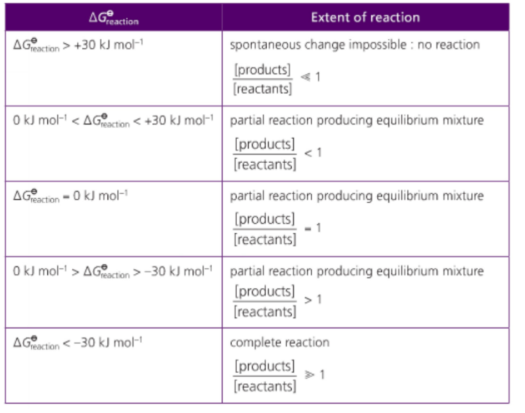
\includegraphics[width=\textwidth]{1.6fig1.png}
	\captionof{figure}{Reaction Limitations created by Gibb's}
\end{figure}

\subsection{Gibbs and Entropy - Spontinuity with Temperature}

\begin{figure}[H]
	\centering
	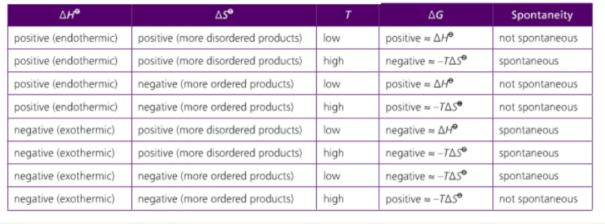
\includegraphics[width=\textwidth]{1.6fig2.png}
	\captionof{figure}{Spontinuity relating to Gibb's and Entropy depending on Temperature}
\end{figure}


\section{Important Side Note}

\begin{enumerate}
\item When compounds change states, $\triangle{G} = 0$ because there is \textbf{no new creation of a product and thus, Gibb's has no real impact}.
\end{enumerate}

\pagebreak






\section{Examples}

\subsection{Find Temp and if Reaction is Spont}

$$\ce{C2H4 + 3O2 -> 2CO2 + 2H2O}$$

\textbf{Solve for Enthalpy First}

\begin{align*}
\triangle{H} 			& = \sum{\triangle{H}_{pro}} - \sum{\triangle{H}_{rea}}\\
\triangle{H} 			&= [(2*-393.5) + (2*-231.8)] - [52 - 3(0)]\\
\triangle{H}			& = -1322.6kJ/mol
\end{align*}

\textbf{Next solve for Entropy}

\begin{align*}
\triangle{S} 		&= \sum{\triangle{S}_{pro}} - \sum{\triangle{S}_{rea}}\\
\triangle{S} 		&= [(2*213.8) + (2*188.8)] - [220 + 3*205]\\
\triangle{S} 		&= -29.8 J/molK
\end{align*}

\textbf{Solve for Gibb's Free Energy}

\begin{align*}
\triangle{G} 		&= \sum{\triangle{G}_{pro}} - \sum{\triangle{G}_{rea}}\\
\triangle{G} 		&= [(2*-394.4) + (2*-228.6)] - [68 + 0]\\
\triangle{G} 		&= -1314kJ/mol
\end{align*}

\textbf{Now we can solve for the temperature!}

\begin{align*}
\triangle{G} 		&= \triangle{H} - T*\triangle{S}\\
T 				&= \frac{\triangle{H} - \triangle{G}}{\triangle{S}}\\
T 				&= 288.6K
\end{align*}

$\boxed{\therefore \ce{the reaction is spontaneous bc} \triangle{G} < 0}$

\subsection{$\star\ce{IMPORATNT}$ Finding Temperature Range for a reaction to take place}

What is the temperature range of a reactino that has an enthalpy of -426kJ/mol and entropy of 109J/molK.

Whenever asked to find the temperature range, we solve two equations. One where $\triangle{G} > 0\ and\ < 0$ to find the \underline{max range} where the reaction is \underline{partially reacted}.


\textbf{Step 1 - Definte a system to solve}

As stated above, we need to find the temperature range. The range is limited at $\triangle{G} =$-30kJ/mol and 30kJ/mol. This is because of the chart shown above in Section 4.1. Based off that chart, the range for spontaneous reactions is -30 to 30.

\textbf{Solving for 1st equation}

\begin{align*}
T &= \frac{\triangle{H} - \triangle{G}}{\triangle{S}}\\
T &= \frac{-426 - 30}{0.109}\\
T &= 3633K
\end{align*}

\textbf{Solving for 2nd equation}

\begin{align*}
T &= \frac{triangle{H} - \triangle{G}}{\triangle{S}}\\
T &= \frac{-426 - (-30)}{0.109}\\
T &= 4283K
\end{align*}

$\boxed{\ce{Therefore the range for which a spontaneous reaction will occur is from} 3633K ~ 4283K}$


















\end{document}
